\documentclass[aspectratio=169,11pt]{beamer}

\usetheme{default}
\usecolortheme{default}
\setbeamertemplate{navigation symbols}{}
\setbeamertemplate{footline}[frame number]
\definecolor{accent}{HTML}{2A78D6}
\definecolor{accent2}{HTML}{EB6834}
\setbeamercolor{frametitle}{fg=accent}
\setbeamercolor{title}{fg=accent}
\setbeamercolor{structure}{fg=accent}
\setbeamerfont{frametitle}{series=\bfseries}

\usepackage{booktabs}
\usepackage{graphicx}
\usepackage{amsmath}

\graphicspath{{../results/figures/}}
\newcommand{\LRTestPRAUC}{0.461}
\newcommand{\XGBTestPRAUC}{0.468}
\newcommand{\LRTestROCAUC}{0.640}
\newcommand{\XGBTestROCAUC}{0.645}
\newcommand{\RouteTestPRAUC}{0.381}
\newcommand{\PriorTestPRAUC}{0.335}
\newcommand{\LRValPRAUC}{0.297}
\newcommand{\XGBValPRAUC}{0.276}
\newcommand{\LRTestRecallThr}{0.031}
\newcommand{\XGBTestRecallThr}{0.035}
\newcommand{\LRTestPrecThr}{0.612}
\newcommand{\XGBTestPrecThr}{0.661}
\newcommand{\LRTestRecallPfifty}{0.276}
\newcommand{\XGBTestRecallPfifty}{0.292}
\newcommand{\XGBRawECE}{0.073}
\newcommand{\XGBCalECE}{0.102}
\newcommand{\XGBRollECE}{0.047}
\newcommand{\LRRawECE}{0.064}
\newcommand{\LRCalECE}{0.103}
\newcommand{\LRRollECE}{0.045}
\newcommand{\XGBMeanPredCal}{0.234}
\newcommand{\XGBRollPRAUC}{0.450}
\newcommand{\XGBRollRecallThr}{0.062}
\newcommand{\XGBRollPrecThr}{0.585}
\newcommand{\LRRollRecallThr}{0.014}
\newcommand{\LRRollPrecThr}{0.557}
\newcommand{\XGBRollWindow}{28}
\newcommand{\LRRollWindow}{28}
\newcommand{\TestRate}{0.335}
\newcommand{\ValRate}{0.178}
\newcommand{\TrainRate}{0.250}
\newcommand{\LRTrainPRAUC}{0.452}
\newcommand{\XGBTrainPRAUC}{0.526}
\newcommand{\LRTrainROCAUC}{0.710}
\newcommand{\XGBTrainROCAUC}{0.752}
\newcommand{\LRValROCAUC}{0.664}
\newcommand{\XGBValROCAUC}{0.650}
\newcommand{\LRC}{10}
\newcommand{\XGBDepth}{4}
\newcommand{\XGBMinChild}{2000}
\newcommand{\XGBLambda}{20}
\newcommand{\XGBTrees}{308}
\newcommand{\NTrain}{244{,}737}
\newcommand{\NVal}{55{,}589}
\newcommand{\NTest}{27{,}020}

\newcommand{\RSFlagged}{1{,}979}
\newcommand{\RSMoved}{133}
\newcommand{\RSEarlier}{98}
\newcommand{\RSRiskBefore}{0.571}
\newcommand{\RSRiskAfter}{0.510}
\newcommand{\RSExpBefore}{1123}
\newcommand{\RSExpAfter}{1115}
\newcommand{\RSFlaggedRate}{0.520}


\title{Day-Ahead Flight Delay Risk Prediction}
\subtitle{Phase 1: Machine Learning}
\author{Member 1 \and Member 2 \and Member 3 \and Member 4 \and Member 5}
\institute{Advanced Machine Learning Course Project}
\date{}

\begin{document}

\begin{frame}
\titlepage
\end{frame}

%---------------------------------------------------------------
\begin{frame}{Problem}
\begin{itemize}
\item Predict on the \textbf{night before departure} whether a flight from NYC will arrive
  \textbf{15+ minutes late} (BTS definition).
\item Output: a calibrated delay probability, plus an offline what-if rescheduling rule.
\item Allowed information at decision time:
  \begin{itemize}
  \item the published schedule of the day (carrier, route, times, aircraft)
  \item outcomes of \emph{strictly earlier} days
  \end{itemize}
\item Not allowed: departure delay, actual times, air time, anything from the same day.
\end{itemize}
\vspace{0.4em}
\[
P\big(y_i = 1 \mid \{s_j : d_j = d_i\} \cup \{(s_j, y_j) : d_j < d_i\}\big)
\]
\end{frame}

%---------------------------------------------------------------
\begin{frame}{Dataset: NYC flights 2013}
\begin{columns}[T]
\column{0.5\textwidth}
\begin{itemize}
\item 336,776 departures from EWR, JFK, LGA
\item 16 carriers, 105 destinations, 4,043 aircraft
\item 8,255 cancelled + 1,175 diverted\\$\Rightarrow$ no label, excluded as examples\\
  (still counted in scheduled volume)
\item 24.5\% delayed 15+ min
\item corr(dep\_delay, arr\_delay) = 0.915\\$\Rightarrow$ post-departure fields removed
\end{itemize}
\column{0.5\textwidth}
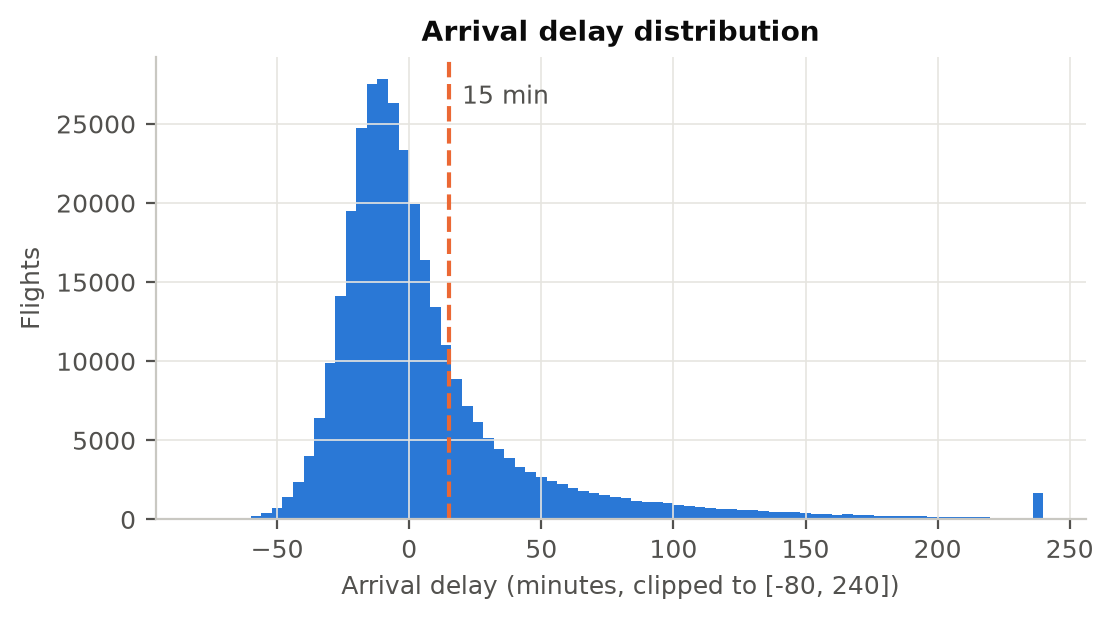
\includegraphics[width=\linewidth]{eda_arr_delay.png}
\end{columns}
\end{frame}

%---------------------------------------------------------------
\begin{frame}{EDA: strong seasonality and a shifted test month}
\begin{columns}[c]
\column{0.55\textwidth}
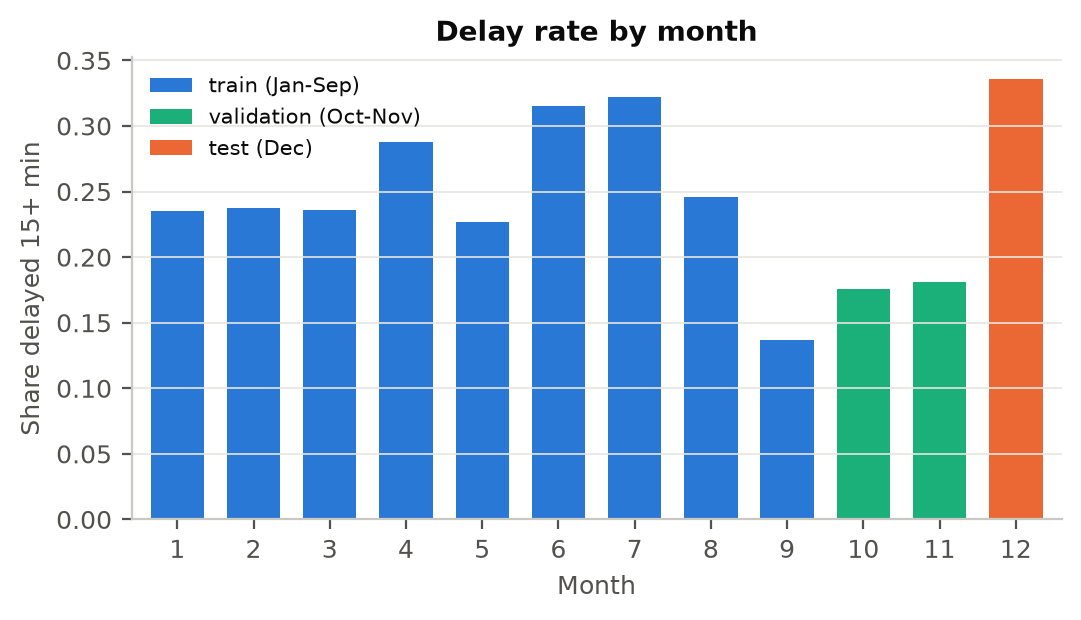
\includegraphics[width=\linewidth]{eda_month.png}
\column{0.45\textwidth}
\begin{itemize}
\item Chronological split:\\
  train Jan--Sep, val Oct--Nov, test Dec
\item Base rate: train \TrainRate, val \ValRate, test \TestRate
\item Test month is the worst of the year, validation among the calmest
\item No month / day-of-year features: Oct--Dec never appear in training
\end{itemize}
\end{columns}
\end{frame}

%---------------------------------------------------------------
\begin{frame}{EDA: time of day and day-to-day persistence}
\centering
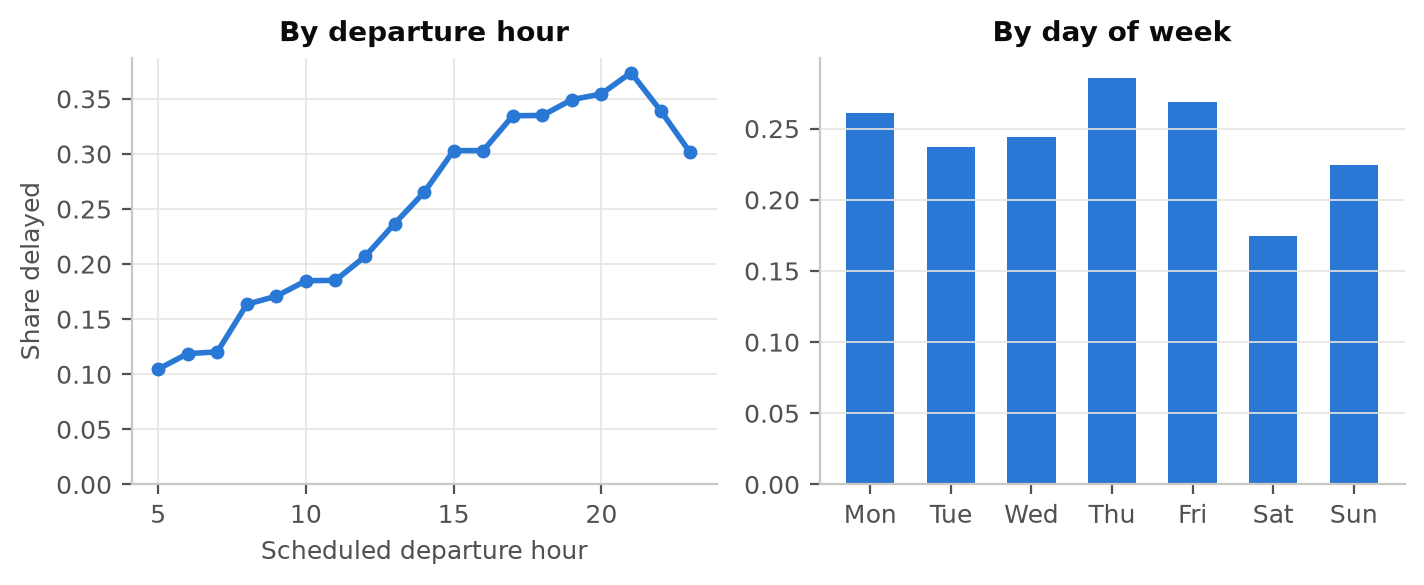
\includegraphics[width=0.49\textwidth]{eda_hour_dow.png}\hfill
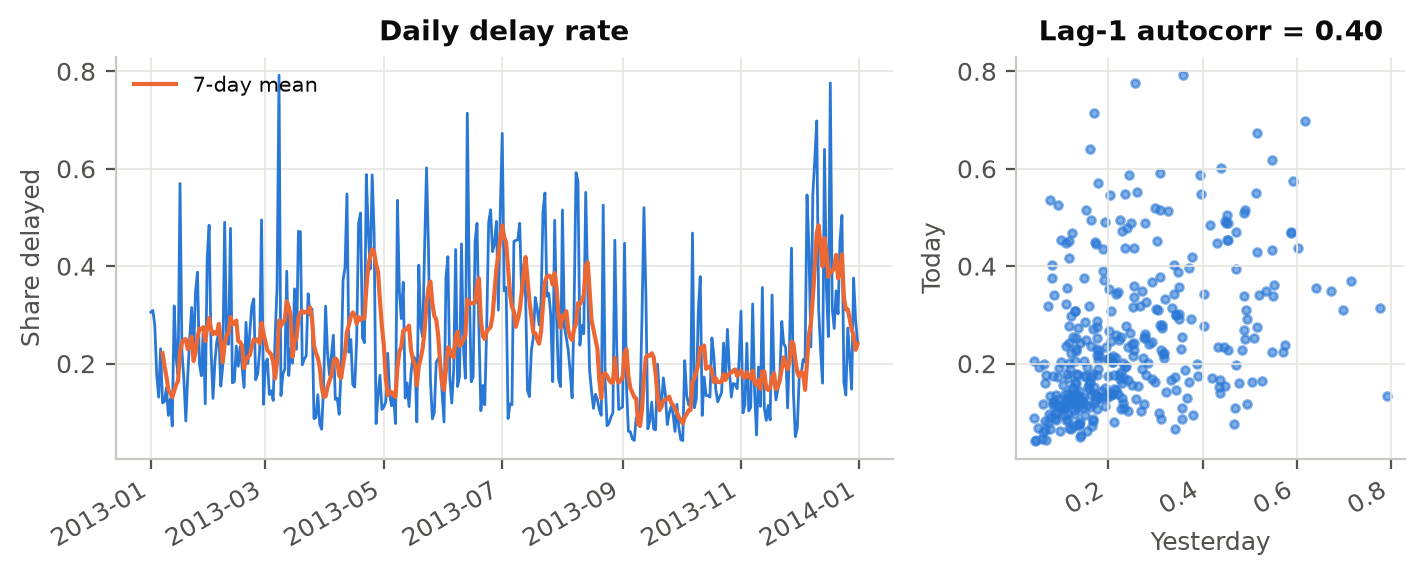
\includegraphics[width=0.49\textwidth]{eda_daily.png}
\begin{itemize}
\item Delay rate climbs from 10.5\% (05:00) to 37\% (21:00): delays propagate through the day
\item Lag-1 autocorrelation of the daily delay rate 0.40, lag-2 only 0.13
\end{itemize}
\end{frame}

%---------------------------------------------------------------
\begin{frame}{Feature engineering (35 features)}
\small
\begin{tabular}{p{0.2\textwidth}p{0.72\textwidth}}
\toprule
Calendar & cyclic time of day (dep/arr), cyclic day of week, weekend, days to holiday \\
Schedule & departure hour, distance, overnight arrival; carrier, origin, dest \\
Congestion & scheduled flights per origin-day / origin-hour / dest-day / carrier-day; aircraft's legs today and leg number \\
Long-run history & smoothed past delay rate per carrier, origin, dest, route, carrier-route, origin-hour, flight no., aircraft \\
Recent history & 7-day rates; yesterday's system/origin delay rate, cancellations, mean delay \\
\bottomrule
\end{tabular}
\vspace{0.5em}
\begin{itemize}
\item Past-only sums $K_g(d) = \sum_{d'<d} k_g(d')$, smoothed:
  $\hat r_g = \dfrac{K_g + m\,p_0}{N_g + m}$, $m = 20$
\item \textbf{Leakage test:} scramble all outcomes from a cutoff date on $\Rightarrow$ features up to the cutoff must not change
\end{itemize}
\end{frame}

%---------------------------------------------------------------
\begin{frame}{Models and theory}
\begin{columns}[T]
\column{0.5\textwidth}
\textbf{Logistic regression}
\begin{itemize}
\item L2-regularised log-loss, convex
\item Intercept optimum $\Rightarrow \sum p_i = \sum y_i$ (calibrated in the large)
\item One-hot categoricals, standardised numerics; $C = \LRC$
\end{itemize}
\column{0.5\textwidth}
\textbf{XGBoost}
\begin{itemize}
\item 2nd-order boosting, $g = p - y$, $h = p(1-p)$
\item Leaf $w^* = -G/(H+\lambda)$
\item \texttt{min\_child\_weight} = \XGBMinChild: $H \ge 2000$, $h \le \tfrac14$ $\Rightarrow$ $\ge$ 8,000 flights per leaf
\item depth \XGBDepth, $\lambda = \XGBLambda$, \XGBTrees{} trees (early stopping)
\end{itemize}
\end{columns}
\vspace{0.6em}
\textbf{Calibration:} Platt $q = \sigma(a\,\mathrm{logit}\,p + c)$ fitted on Oct--Nov, and a \emph{rolling} Platt
refitted daily on the last \XGBRollWindow{} days (window chosen on November).
\end{frame}

%---------------------------------------------------------------
\begin{frame}{Results on December (test)}
\begin{columns}[c]
\column{0.62\textwidth}
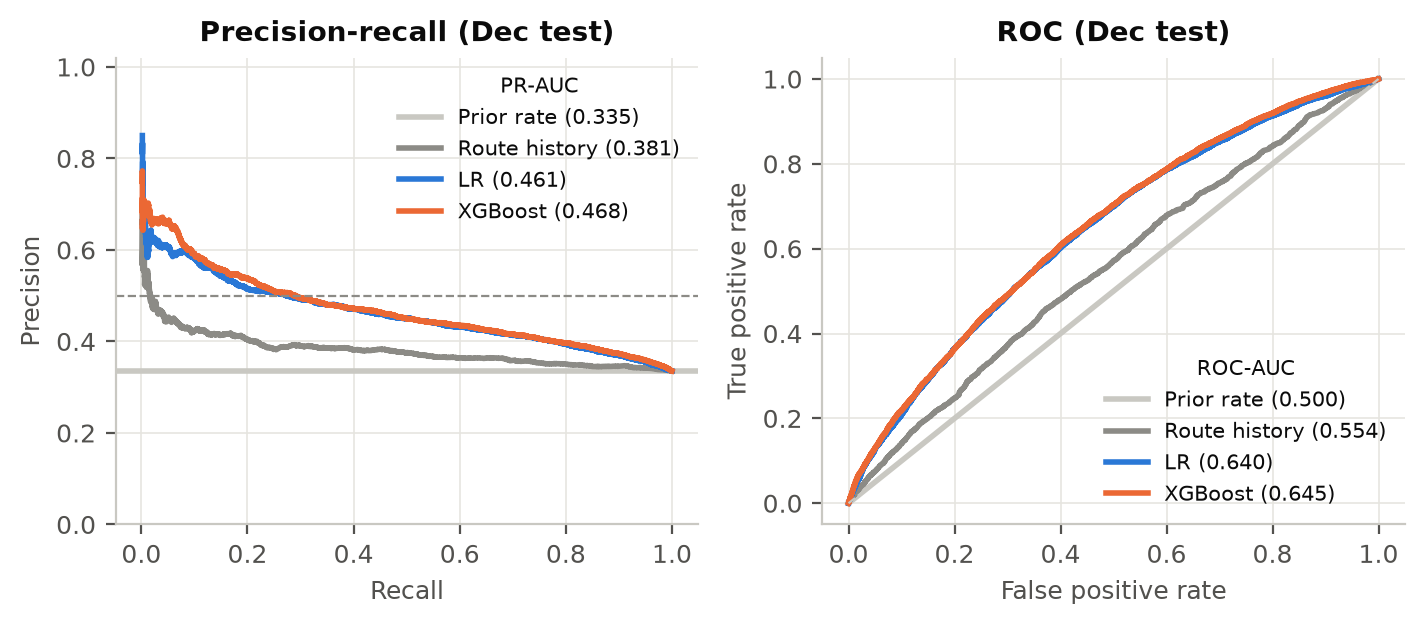
\includegraphics[width=\linewidth]{pr_roc_test.png}
\column{0.38\textwidth}
\footnotesize
\resizebox{\linewidth}{!}{\begin{tabular}{lcccc}
\toprule
Model & PR-AUC & ROC-AUC & Brier & ECE \\
\midrule
Prior rate & 0.335 & 0.500 & 0.230 & 0.086 \\
Route history & 0.381 & 0.554 & 0.230 & 0.095 \\
LR & 0.461 & 0.640 & 0.222 & 0.103 \\
XGBoost & 0.468 & 0.645 & 0.221 & 0.102 \\
\bottomrule
\end{tabular}
}
\vspace{0.6em}
\begin{itemize}
\item Both models beat route history
\item XGB $\approx$ LR on test;\\LR better on validation (\LRValPRAUC{} vs \XGBValPRAUC)
\end{itemize}
\end{columns}
\end{frame}

%---------------------------------------------------------------
\begin{frame}{Why XGBoost needed heavy regularisation}
\begin{itemize}
\item Train vs validation ROC-AUC: XGBoost \XGBTrainROCAUC{} $\to$ \XGBValROCAUC, LR \LRTrainROCAUC{} $\to$ \LRValROCAUC
\item Day-level features (yesterday's rates) are constant within a day $\Rightarrow$ together they fingerprint the date
\item Small leaves let trees memorise the weather of individual training days
\item Validation picked the largest \texttt{min\_child\_weight}: every leaf spans $\sim$9 days of flights
\item Day-of-year features removed for the same reason
\end{itemize}
\end{frame}

%---------------------------------------------------------------
\begin{frame}{Class imbalance: we tried class weighting}
\centering
\resizebox{0.9\textwidth}{!}{\begin{tabular}{lccccc}
\toprule
Model & Val PR-AUC & Test PR-AUC & Test ROC-AUC & Test ECE & Mean $\hat p$ \\
\midrule
LR (unweighted) & 0.297 & 0.461 & 0.640 & 0.064 & 0.295 \\
LR, balanced class weights & 0.296 & 0.460 & 0.641 & 0.182 & 0.517 \\
XGBoost (unweighted) & 0.276 & 0.468 & 0.645 & 0.073 & 0.269 \\
XGBoost, positive weight 3.00 & 0.273 & 0.466 & 0.647 & 0.153 & 0.488 \\
\bottomrule
\end{tabular}
}
\vspace{0.8em}
\begin{itemize}
\item 25\% of training flights delayed: moderate imbalance
\item Weighting barely changes PR-AUC / ROC-AUC
\item But it inflates probabilities (mean $\hat p \approx 0.5$ vs observed \TestRate) and more than doubles ECE
\item Kept unweighted; imbalance handled by PR-AUC + precision-based threshold
\item No SMOTE: synthetic flights mixing different days break day-level history features
\end{itemize}
\end{frame}

%---------------------------------------------------------------
\begin{frame}{Calibration breaks under the base-rate shift}
\begin{columns}[c]
\column{0.6\textwidth}
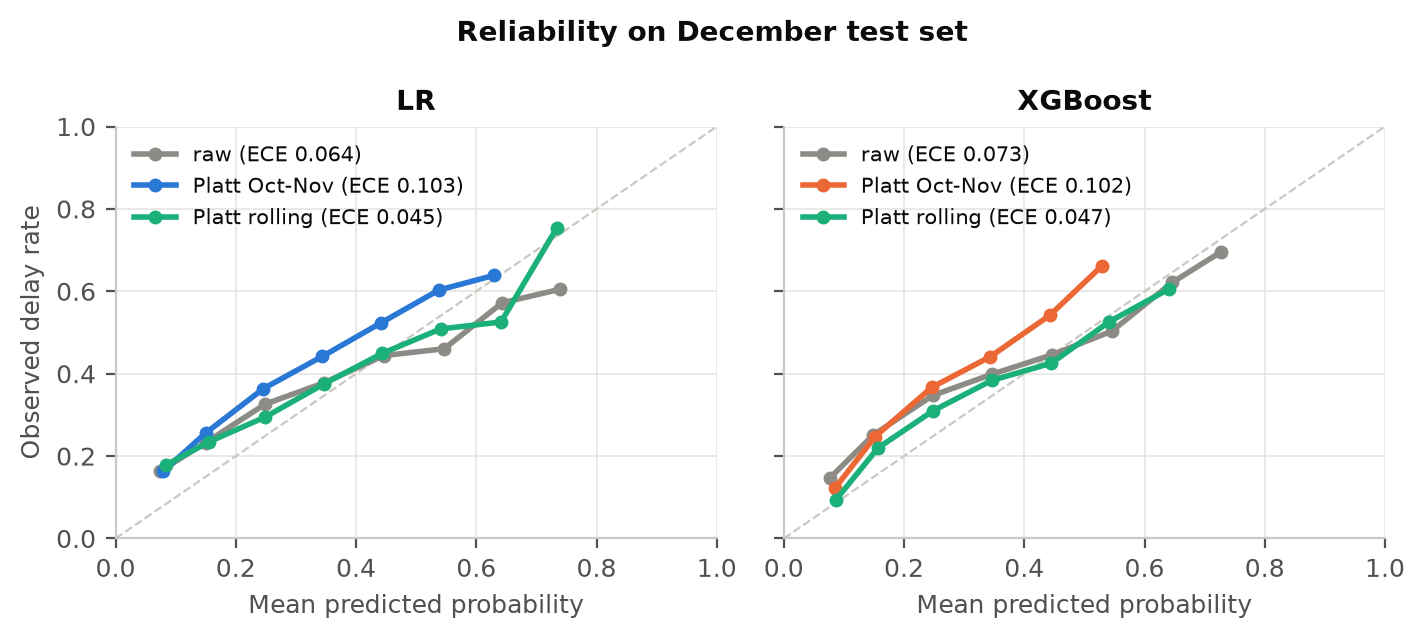
\includegraphics[width=\linewidth]{reliability_test.png}
\column{0.4\textwidth}
\begin{itemize}
\item Oct--Nov Platt learns a low base rate $\Rightarrow$ under-predicts December
\item ECE (XGB): raw \XGBRawECE, fixed \XGBCalECE, \textbf{rolling \XGBRollECE}
\item Label shift theory: only the intercept needs to follow $\log\frac{\pi}{1-\pi}$
\item Cost: pooled PR-AUC \XGBRollPRAUC
\end{itemize}
\end{columns}
\end{frame}

%---------------------------------------------------------------
\begin{frame}{Operating point: precision $\ge 0.5$}
\centering
\begin{tabular}{lcccc}
\toprule
Model & Threshold & Flagged & Precision & Recall \\
\midrule
LR & 0.519 & 1.7\% & 0.612 & 0.031 \\
XGBoost & 0.498 & 1.8\% & 0.661 & 0.035 \\
LR (rolling cal.) & 0.648 & 0.9\% & 0.557 & 0.014 \\
XGBoost (rolling cal.) & 0.576 & 3.6\% & 0.585 & 0.062 \\
\bottomrule
\end{tabular}

\vspace{0.8em}
\begin{itemize}
\item Threshold chosen on validation, applied unchanged to December
\item Precision holds, recall is low: the shift makes December scores look ``too low''
\item Reference only (read off the test curve): recall at precision $\ge 0.5$ = \XGBTestRecallPfifty{} (XGB), \LRTestRecallPfifty{} (LR)
\end{itemize}
\end{frame}

%---------------------------------------------------------------
\begin{frame}{Feature ablation and importance}
\begin{columns}[c]
\column{0.62\textwidth}
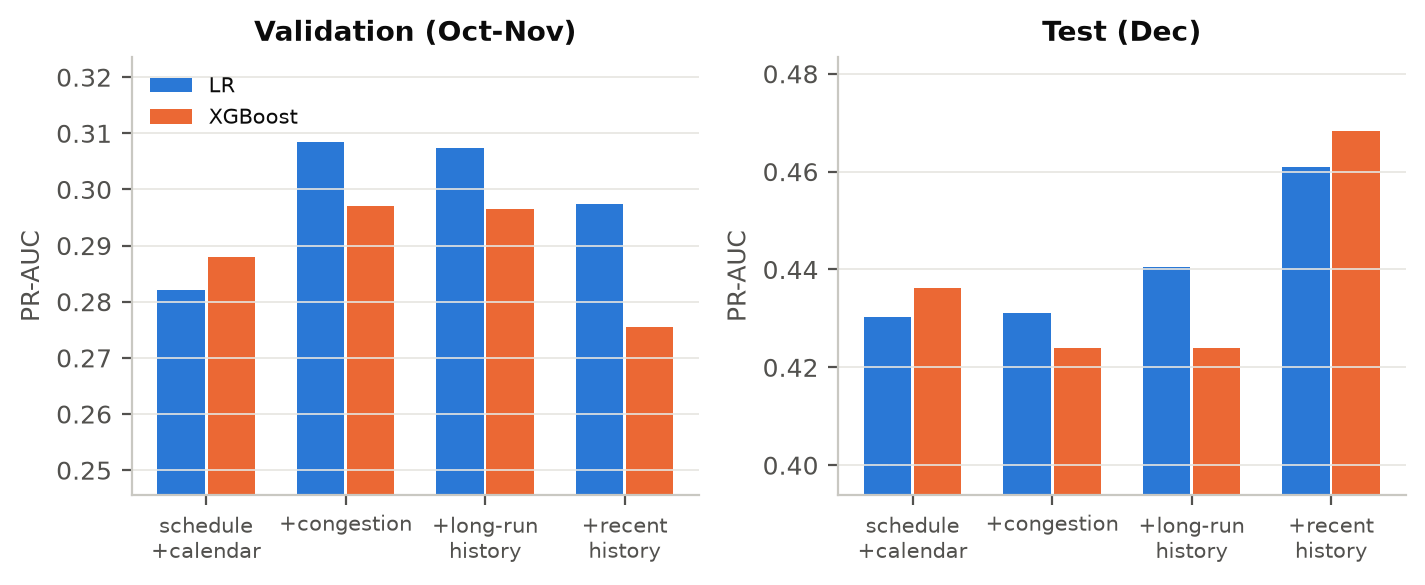
\includegraphics[width=\linewidth]{ablation.png}
\column{0.38\textwidth}
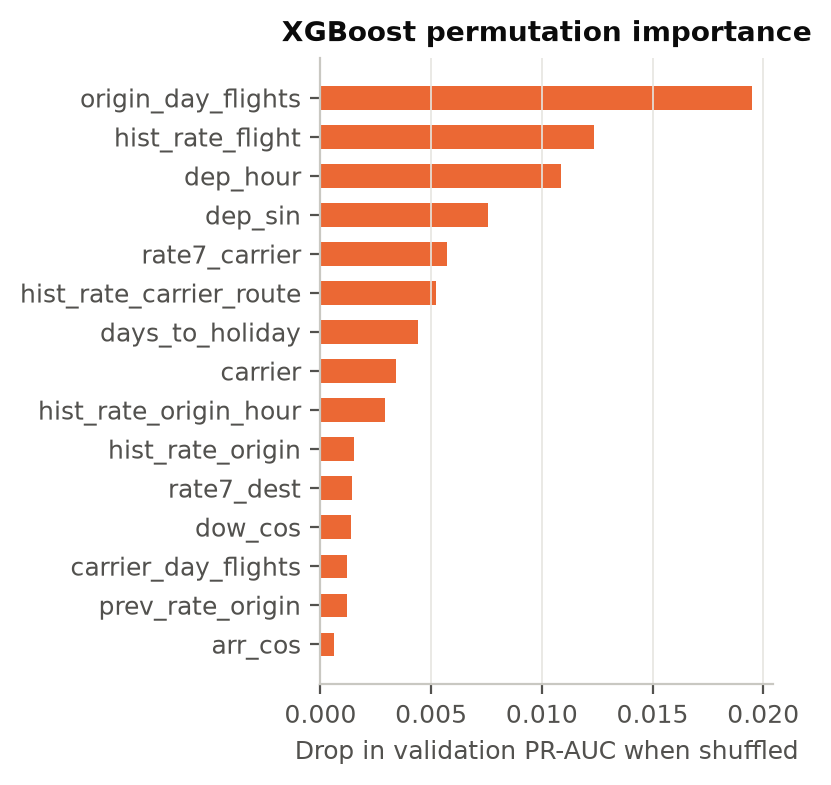
\includegraphics[width=\linewidth]{permutation_importance.png}
\end{columns}
\begin{itemize}
\item Congestion helps most on calm validation months
\item Recent history hurts slightly on validation but is the biggest gain on December
\end{itemize}
\end{frame}

%---------------------------------------------------------------
\begin{frame}{What-if rescheduling (December, LR + rolling calibration)}
\begin{columns}[c]
\column{0.55\textwidth}
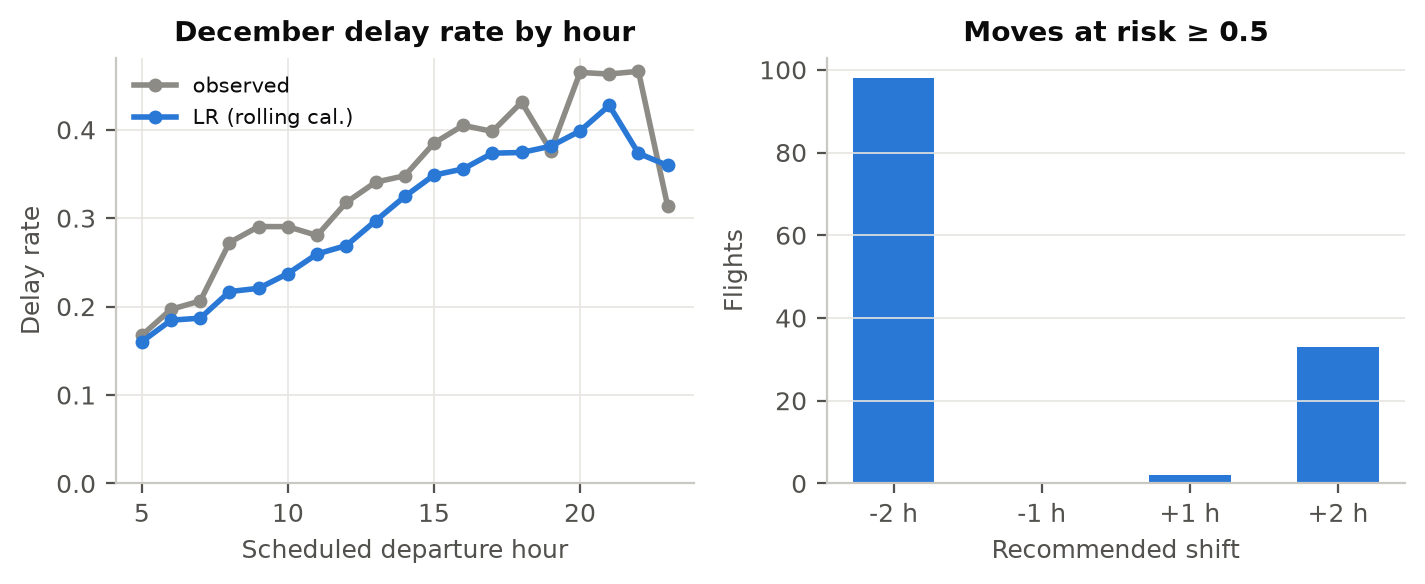
\includegraphics[width=\linewidth]{reschedule.png}
\column{0.45\textwidth}
\small
\begin{itemize}
\item Risk $\ge 0.5$ $\Rightarrow$ try $\pm1$, $\pm2$ h same day; move if risk drops $\ge 0.05$, max 3 moved flights per origin-hour
\item \RSFlagged{} flagged, \RSMoved{} moved (\RSEarlier{} earlier)
\item Moved flights: risk \RSRiskBefore{} $\to$ \RSRiskAfter
\item Expected delays among flagged: \RSExpBefore{} $\to$ \RSExpAfter
\item Associational, ignores crews, rotations, connections
\end{itemize}
\end{columns}
\end{frame}

%---------------------------------------------------------------
\begin{frame}{Limitations and Phase 2}
\begin{itemize}
\item No weather forecast: day-level weather dominates and caps day-ahead accuracy
\item One year, NYC departures only: inbound legs and Oct--Dec seasonality unseen
\item Cancelled/diverted flights dropped (cluster on the worst days)
\item Rescheduling estimate is not causal
\end{itemize}
\vspace{0.6em}
\textbf{Phase 2:} compact MLP with learned embeddings for carrier, origin and destination, same split and features, same metrics.
\end{frame}

%---------------------------------------------------------------
\begin{frame}{Summary}
\begin{itemize}
\item Leakage-free day-ahead pipeline, verified by an automated test
\item December PR-AUC \LRTestPRAUC{} (LR) / \XGBTestPRAUC{} (XGB) vs base rate \TestRate
\item XGBoost only competitive once forced to use large leaves
\item Calibration must adapt to drift: rolling Platt cuts ECE from \XGBCalECE{} to \XGBRollECE
\item Rescheduling: earlier is better, but gains within $\pm2$ h are small
\end{itemize}
\vspace{1em}
\centering
\textbf{Thank you}
\end{frame}

\end{document}
